\chapter{Efficiënte zoekbomen}

\section{Inleiding}
\begin{itemize}
    \item Uitvoeringstijd van operaties op een binaire zoekboom met hoogte $h$ is $O(h)$.
    \item De hoogte $h$ is afhankelijk van de toevoegvolgorde:
    \begin{itemize}
        \item In het slechtste geval bekomt men een gelinkte lijst, zodat $h = O(n)$.
        \item Als elke toevoegvolgorde even waarschijnlijk is, dan is de verwachtingswaarde voor de hoogte $h = O(\lg n)$ met $n$ het aantal gegevens.
        \begin{itemize}
            \alert Geen realistische veronderstelling.
        \end{itemize}
    \end{itemize}
    \item Drie manieren om de efficiëntie van zoekbomen te verbeteren:
    \begin{enumerate}
        \item \textbf{Elke operatie steeds efficiënt maken.}
        \begin{enumerate}
            \item AVL-bomen.
            \begin{itemize}
                \item Hoogteverschil $\Delta h$ van de twee deelbomen van elke knoop is kleiner of gelijk aan 1.
                \item $\Delta h$ wordt opgeslagen in de knoop zelf.
                \begin{figure}[ht]
                    \centering
                    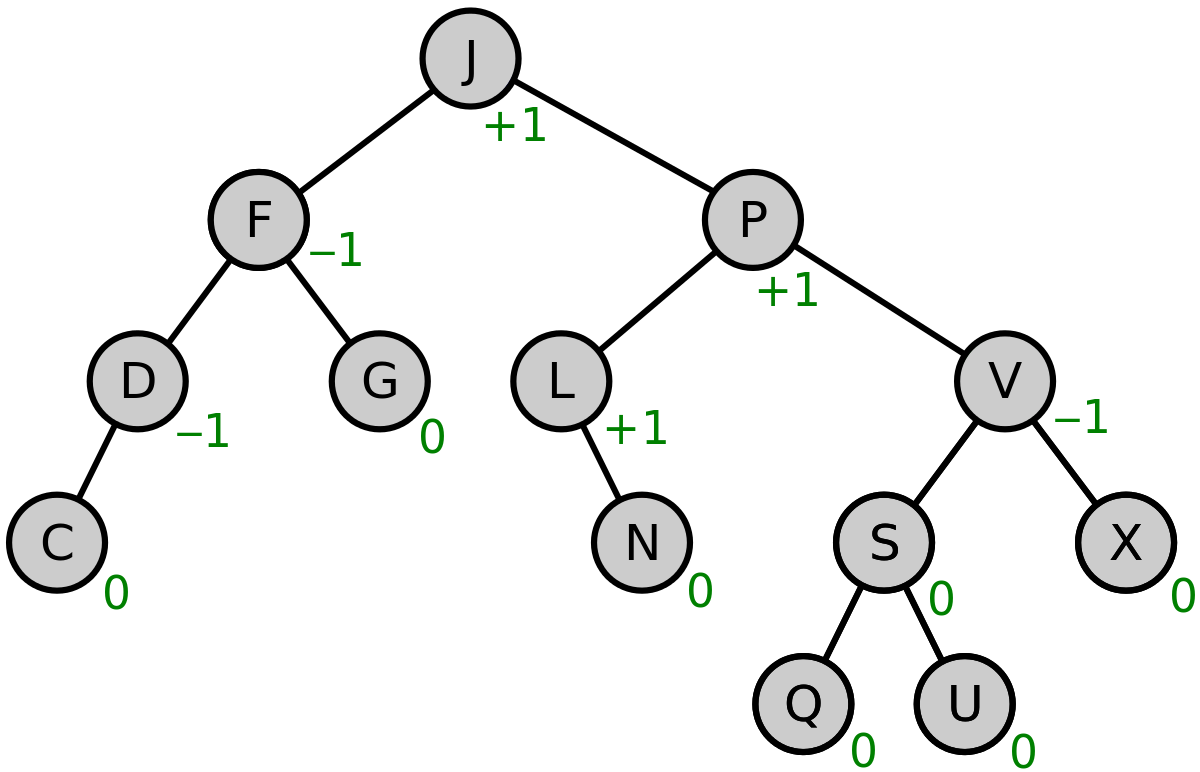
\includegraphics[width=0.5\textwidth]{AVL-tree}
                    \caption{Een AVL-boom. De groene cijfers stellen de hoogteverschillen voor van de twee deelbomen voor elke knoop.}
                    \label{fig:AVL-tree}
                \end{figure}
            \end{itemize}
            \item 2-3-bomen.
            \begin{itemize}
                \item Elke knoop heeft 2 of 3 kinderen.
                \item Elk blad heeft dezelfde diepte.
                \item Bij toevoegen of verwijderen wordt het ideale evenwicht behouden door het aantal kinderen van de knopen te manipuleren.
            \end{itemize}
            \item 2-3-4-bomen.
            \begin{itemize}
                \item Eenvoudiger dan 2-3-bomen om te implementeren.
            \end{itemize}
            \item Rood-zwarte bomen (sectie \ref{sec:rood-zwarte bomen}).
        \end{enumerate}

        \item \textbf{Elke reeks operaties steeds efficiënt maken.}
        \begin{enumerate}
            \item Splaybomen (sectie \ref{sec:splaybomen}).
            \begin{itemize}
                \item De vorm van de boom wordt meermaals aangepast.
                \item Elke reeks opeenvolgende operaties is gegarandeerd efficiënt.
                \item Een individuele operatie kan wel traag uitvallen.
                \item \textit{Geamortiseerd} is de performantie per operatie goed.
            \end{itemize}
        \end{enumerate}

        \item \textbf{De gemiddelde efficiëntie onafhankelijk maken van de operatievolgorde.}
        \begin{enumerate}
            \item Gerandomiseerde zoekbomen (sectie \ref{sec:gerandomiseerde-zoekbomen}).
            \begin{itemize}
                \item Gebruik van een random generator.
                \item De boom is random, onafhankelijk van de toevoeg- en verwijdervolgorde.
                \item Verwachtingswaarde van de hoogte $h$ wordt dan $O(\lg n)$.
            \end{itemize}
        \end{enumerate}
    \end{enumerate}
\end{itemize}

\section{Rood-zwarte bomen}
\subsection{Definitie en eigenschappen}
\begin{figure}[ht]
    \centering
    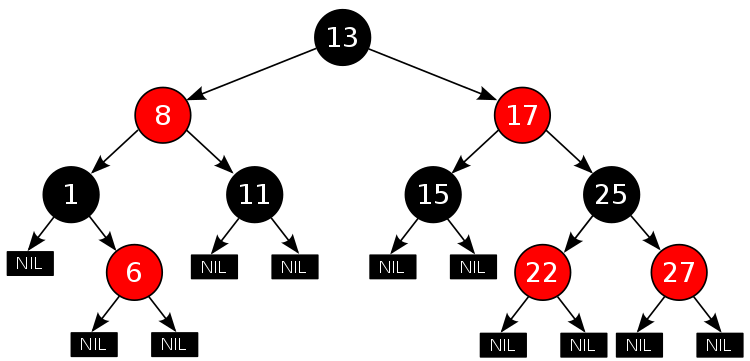
\includegraphics[width=\textwidth]{red-black-tree}
    \caption{Een rood-zwarte boom. De \texttt{NIL} knopen stellen virtuele knopen voor.}
    \label{fig:red-black-tree}
\end{figure}
\label{sec:rood-zwarte bomen}
\begin{itemize}
    \item \textbf{Definitie:}
    \begin{itemize}
        \item Een binaire zoekboom.
        \item Elke knoop is rood of zwart gekleurd.
        \item Elke virtuele knoop is zwart. Een virtuele knoop is een knoop die geen waarde heeft, maar wel een kleur. Deze vervangen de nullwijzers.
        \item Een rode knoop heeft steeds twee zwarte kinderen
        \item Elke mogelijke weg vanuit een knoop naar een virtuele knoop bevat evenveel zwarte knopen. Dit aantal wordt de \textit{zwarte hoogte} genoemd
        \item De wortel is zwart.
    \end{itemize}
    \item \textbf{Eigenschappen:}
    \begin{itemize}
        \item Een deelboom met wortel $w$ en zwarte hoogte $z$ heeft tenminste $2^z - 1$ inwendige knopen.
        \item De hoogte van een rood-zwarte boom met $n$ knopen is steeds $O(\lg n)$.
        \begin{itemize}
            \item Er zijn nooit twee opeenvolgende rode knopen op elke weg vanuit een knoop naar een virtuele knoop $\rightarrow z \geq h/2$.
            \item Substitutie in de eerste eigenschap geeft:
            \begin{align*}
                n &\geq 2^z - 1 \geq 2^{h/2} - 1 \\
                \rightarrow h & \leq 2\lg(n + 1)
            \end{align*}
        \end{itemize}
    \end{itemize}

\end{itemize}
\subsection{Zoeken}
\begin{itemize}
    \item De kleur speelt geen rol, zodat de rood-zwarte boom een gewone binaire zoekboom wordt.
    \item De hoogte is wel gegerandeerd $O(\lg n)$.
    \item Zoeken naar een willekeurige sleutel is dus $O(\lg n)$.
\end{itemize}

\subsection{Toevoegen en verwijderen}
\begin{itemize}
    \item Element toevoegen of verwijderen, zonder rekening te houden met de kleur, is ook $O(\lg n)$.
    \alert Geen garantie dat deze gewijzigde boom nog rood-zwart zal zijn.
    \item Twee manieren om toe te voegen:
    \begin{enumerate}
        \item \textbf{Bottom-up:} 
        \begin{itemize}
            \item Voeg knoop toe zonder rekening te houden met de kleur.
            \item Herstel de rood-zwarte boom, te beginnen bij de nieuwe knoop, en desnoods tot bij de wortel.
        \end{itemize}
        \item \textbf{Top-down:} 
        \begin{itemize}
            \item Pas de boom aan langs de dalende zoekweg.
            \good Efficiënter dan bottom-down aangezien er geen ouderwijzers of een stapel nodig is.
        \end{itemize}
    \end{enumerate}
\end{itemize}

\subsection{Rotaties}
\begin{figure}[ht]
    \centering
    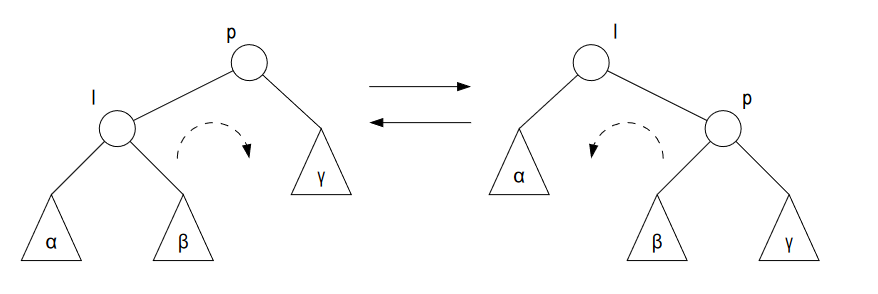
\includegraphics[width=0.5\textwidth]{rotations}
    \caption{Rotaties}
    \label{fig:rotations}
\end{figure}
\begin{itemize}
    \item Wijzigen de vorm van de boom, maar behouden de inorder volgorde van de sleutels.
    \item Moet enkel pointers aanpassen, en is dus $O(1)$.
    \item \textbf{Rechtste rotatie} van een ouder $p$ en zijn linkerkind $l$:
    \begin{itemize}
        \item Het rechterkind van $l$ wordt het linkerkind van $p$.
        \item De ouder van $p$ wordt de ouder van $l$.
        \item $p$ wordt het rechterkind van $l$. 
    \end{itemize}
    \item \textbf{Linkse rotatie} van een ouder $p$ en zijn rechterkind $r$:
    \begin{itemize}
        \item Het linkerkind van $r$ wordt het rechterkind van $p$.
        \item De ouder van $r$ wordt de ouder van $p$.
        \item $p$ wordt het linkerkind van $l$. 
    \end{itemize}
\end{itemize}

\subsection{Bottom-up rood-zwarte bomen}
\todo{vanaf hier}

\subsection{Top-down rood-zwarte bomen}
\section{Splaybomen}
\label{sec:splaybomen}


\section{Gerandomiseerde zoekbomen}
\label{sec:gerandomiseerde-zoekbomen}